\documentclass[twocolumn,amsmath,amssymb,floatfix]{revtex4}

\usepackage{graphicx}% Include figure files
\usepackage{dcolumn}% Align table columns on decimal point
\usepackage{bm}% bold math
\usepackage{amssymb}
\usepackage{amsmath}
\usepackage{amsfonts}
\usepackage{epsf}
\usepackage{color} % allows color in fonts
\usepackage{verbatim}
\usepackage{listings}
\usepackage{xcolor}
\usepackage{titlesec}
\usepackage{float}

\usepackage[brazilian]{babel}
\usepackage[utf8]{inputenc}
\usepackage[T1]{fontenc}

\newcommand{\PAR}[1]{\left({[#1]}\right)}


\lstdefinestyle{customc}{
  belowcaptionskip=1\baselineskip,
  breaklines=true,
  frame=none,
  xleftmargin=\parindent,
  language=C,
  showstringspaces=false,
  basicstyle=\footnotesize\ttfamily,
  keywordstyle=\bfseries\color{green!40!black},
  commentstyle=\itshape\color{purple!40!black},
  identifierstyle=\color{blue},
  stringstyle=\color{orange},
}

\lstdefinestyle{customasm}{
  belowcaptionskip=1\baselineskip,
  frame=trBL,
  xleftmargin=\parindent,
  language=[x86masm]Assembler,
  basicstyle=\footnotesize\ttfamily,
  commentstyle=\itshape\color{purple!40!black},
}

\lstset{escapechar=@,style=customc}

\titlespacing\section{0pt}{12pt plus 4pt minus 2pt}{8pt plus 2pt minus 2pt}
\titlespacing\subsection{0pt}{12pt plus 4pt minus 2pt}{8pt plus 2pt minus 2pt}
\titlespacing\subsubsection{0pt}{12pt plus 4pt minus 2pt}{0pt plus 2pt minus 2pt}

\begin{document}

%%%%%%%%%%%%%%%%%%%%%%
%%%%%%%%%%%%%%%%%%%%%%
% T I T U L O
%%%%%%%%%%%%%%%%%%%%%%
%%%%%%%%%%%%%%%%%%%%%%

\title{Relatorio Exercicio Computacional 2}

\author{Leonardo Heidi Almeida Murakami - NUSP: 11260186 \\\small leonardo.murakami@usp.br} 
\affiliation{
Instituto de Matemática e Estatística - Universidade de São Paulo\\
}

\begin{abstract}
\baselineskip 11pt
Neste trabalho utilizaremos algumas variantes de Monte Carlo, que consiste, no geral, em amostragens aleatórias massivas para obter resultados numéricos. Utilizaremos deste método para estimarmos o valor de uma integral a partir de números aleatórios
\end{abstract}

\maketitle
%%%%%%%%%%%%%%%%%%%%%%
%%%%%%%%%%%%%%%%%%%%%%
\section{Introdução e Conceitos}
%%%%%%%%%%%%%%%%%%%%%%
%%%%%%%%%%%%%%%%%%%%%%

\indent Os métodos de Monte Carlo são uma classe ampla de algoritmos computacionais que dependem de uma amostragem aleatória para obter resultados numéricos. 
\\\indent A ideia para obtermos o valor de 
\begin{eqnarray}
  \int^1_0 exp(0.394353985x)*cos(0.50451412877x)
\end{eqnarray}
sera nos utilizarmos de 4 métodos diferentes de Monte Carlo.
\subsection{Hit or Miss Monte Carlo}
O primeiro dos métodos que utilizamos será semelhante àquele usado no último exercício computacional, o método Hit or Miss consiste em calcularmos a área de uma dada figura (no caso o gráfico da função apresentada acima) através de uma quantidade aleatória de pontos que caem dentro da área desejada sobre a área total, representada por um quadrado 1x1. \\
\indent Com esta proporção é possivel saber a porcentagem do quadrado representada pelo gráfico da função e conseguir uma estimativa da área embaixo do gráfico, vulgo, a integral.
\subsection{Crude Monte Carlo}
\indent O segundo método que estudaremos consiste em utilizarmos uma distribuição uniforme para gerar números aleatórios para obtermos o valor de f(x), que após um número N de amostras acaba gerando uma distribuição muito proxima do formato original do gráfico da função desejada, realiza-se então a média destes valores para calcularmos algo próximo a área embaixo do gráfico.
\subsection{Importance Sampling}
\indent Outro método que utilizaremos em nosso estudo será o Importance Sampling, que consiste em uma tecnica para reduzirmos a variância de um metodo de Monte Carlo, a ideia por traz do importance sampling é de que certos valores aleatórios em uma simulação tem mais impacto no parametro sendo estimado que outros. Porém o uso direto dessa distribuição enviesada resultará em um estimador enviesado se for aplicado diretamente na simulação, por isso os outputs são calculados através de pesos, para garantir que o estimador seja correto\\
\indent Calculamos a estimativa através de:
\begin{eqnarray}
  \hat\gamma_s = \frac{1}{n}\sum_1^n\frac{f(x_i)}{g(x_i)}
\end{eqnarray}
\indent Mostraremos as distribuições utilizadas na seção 2.C deste documento
\subsection{Control Variates}
\indent O ultimo método testado foi o de Control Variates para reduzir a variância do experimento. Esse método explora informação sobre os erros em estimativas que conseguimos calcular para reduzir o erro de estimativas que não conseguimos calcular. \\
\indent No nosso caso, a função usada para reduzir o erro da nossa integral foi
\begin{eqnarray}
  g(x) = -0.4x + 1
\end{eqnarray}
por possuir um valor muito próximo a função que queremos estudar, além de possuir um valor de integral relativamente simples, a comparação das funções no domínio de [0, 1[, proposto pelo exercício esta indicado a baixo pelo gráfico
\\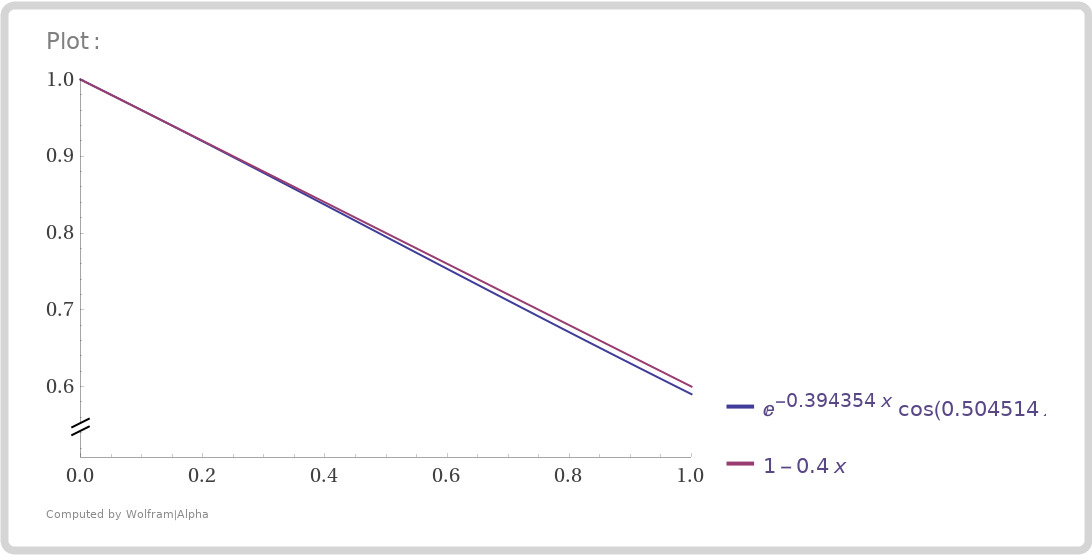
\includegraphics[scale=0.23]{control_variate_graph.jpg}
Calculamos a nossa estimativa através de:
\begin{eqnarray}
  \hat\gamma=\frac{1}{n}\sum_1^nf(x_i)-\phi(x_i)+\gamma'
\end{eqnarray}
onde 
\begin{eqnarray}
 \gamma'=\int_0^1\phi(x)dx
\end{eqnarray}
%%%%%%%%%%%%%%%%%%%%%%
%%%%%%%%%%%%%%%%%%%%%%
\section{Implementação e testes}
%%%%%%%%%%%%%%%%%%%%%%
%%%%%%%%%%%%%%%%%%%%%%

\indent O algoritmo foi implementado na linguagem Python 3.8, organizado em 1 arquivo: monte-carlo-integration.py. \\
\indent Os gráficos foram gerados usando a biblioteca \textit{matplotlib} do Python e utilizando a interface web do \textit{Wolfram|Alpha}, as distribuções foram geradas utilizando a biblioteca \textit{SciPy} e a algebra com vetores foi otimizada utilizando-se da biblioteca \textit{NumPy}. As partes relevantes dos códigos podem ser conferidos no próprio arquivo enviado junto com este PDF/Tex.

%%%%%%%%%%%%%%%%%%%%%%
\subsection{Arquivos do projeto}
%%%%%%%%%%%%%%%%%%%%%%
Abaixo segue um breve resumo do conteúdo dos códigos fonte e interfaces.
\\\indent \textbf{monte-carlo-integration.py:} Implementa todo o algoritmo. Um pedaço de sua interface é apresentado a seguir:
\begin{lstlisting}
def generate_point() -> Tuple(float, float):

def generate_values(dist: Scipy.distribution, size: int=30000) -> List(float):

def crude_monte_carlo(f_x: Function, n_samples: int) -> float:

def hit_or_miss_monte_carlo(f_x: Function, n_samples: int) -> float:

def importance_sampling_monte_carlo(distribution: Scipy.distribution, f_x: Function, n_samples: int) -> float:

def control_variates_monte_carlo(control_variate: Function, gamma_integrated_control_variate: float, f_x: Function, n_samples: int) -> float:

def estimate_error(monte_carlo_algorithm: function, f_x: function, n_batches: int, distribution: Scipy.distribution, control_variate: function, gamma_integrated_control_variate: float) -> List(float), float:

def main() -> None
\end{lstlisting}
%%%%%%%%%%%%%%%%%%%%%%
\subsection{Algoritmo}
%%%%%%%%%%%%%%%%%%%%%%
\indent A implementação do algoritmo em questão é apresentado abaixo. As funções com o nome de monte\_carlo são passadas como argumento para a função estimate\_error que recebe como argumento os argumentos necessarios para que todos os metodos de Monte Carlo rodem com sucesso, os $N$ foram definidos como constantes no começo do código assim como o valor $M$, que é o numero de vezes que cada algoritmo de Monte Carlo ira rodar para podermos calcular um erro
\begin{lstlisting}
def main():
  errors_crude, estimated_value_crude = estimate_error(crude_monte_carlo, f_x)
  print("-"*4 + "CRUDE MONTE CARLO" + "-"*4)
  print(f"Mean Error: \t {np.mean(errors_crude)}")
  print(f"Estimated Value: \t {estimated_value_crude}")

  errors_hom, estimated_value_hom = estimate_error(hit_or_miss_monte_carlo, f_x)
  print("-"*4 + "HIT OR MISS MONTE CARLO" + "-"*4)
  print(f"Mean Error: \t {np.mean(errors_hom)}")
  print(f"Estimated Value: \t {estimated_value_hom}")

  isc_errors, isc_estimated_value = estimate_error(importance_sampling_monte_carlo, f_x, distribution=stats.beta(a=1, b=1.2))
  print("-"*4 + "BETA DISTRIBUTION IMPORTANCE SAMPLING MONTE CARLO" + "-"*4)
  print(f"Mean Error: \t {np.mean(isc_errors)}")
  print(f"Estimated Value: \t {isc_estimated_value}")

  isc_errors, isc_estimated_value = estimate_error(importance_sampling_monte_carlo, f_x, distribution=stats.gamma(a=1, scale=1.4))
  print("-"*4 + "GAMMA DISTRIBUTION IMPORTANCE SAMPLING MONTE CARLO" + "-"*4)
  print(f"Mean Error: \t {np.mean(isc_errors)}")
  print(f"Estimated Value: \t {isc_estimated_value}")

  isc_errors, isc_estimated_value = estimate_error(importance_sampling_monte_carlo, f_x, distribution=stats.weibull_min(c=1, scale=1.1))
  print("-"*4 + "WEIBULL DISTRIBUTION IMPORTANCE SAMPLING MONTE CARLO" + "-"*4)
  print(f"Mean Error: \t {np.mean(isc_errors)}")
  print(f"Estimated Value: \t {isc_estimated_value}")
  
  control_variate = lambda x: -0.4*x + 1
  gamma_integrated_control_variate = 0.8
  control_variate_errors, control_variate_estimated_value = estimate_error(
      control_variates_monte_carlo, f_x, 
      control_variate = control_variate,
      gamma_integrated_control_variate = gamma_integrated_control_variate
      )
  print("-"*4 + "CONTROL VARIATES MONTE CARLO" + "-"*4)
  print(f"Mean Error: \t {np.mean(control_variate_errors)}")
  print(f"Estimated Value: \t {control_variate_estimated_value}")
\end{lstlisting}
\indent A função main é utilizada para rodarmos todos os algoritmos dentro da função estimate error para gerarmos os valores estimados e erros, todos os atributos de distribuições, assim como a função do metodo Control Variates estão definidos dentro da main e podem ser alterados sem muita dificuldade
%%%%%%%%%%%%%%%%%%%%%%
\subsection{Distribuições Escolhidas}
%%%%%%%%%%%%%%%%%%%%%%
\indent Para podermos realizar a redução de variância do método de Importance Sampling, precisávamos de um método de escolher os parâmetros das distribuições indicadas pelo enunciado do exercício, sendo elas as distribuições Beta, Gamma e Weibull.\\
\indent Através de iterações manuais alterando os parametros, encontrei distribuições que mostravam-se relativamente proximas a curva gerada pela função que queriamos integrar, abaixo temos os graficos comparando ambas as curvas
\subsubsection{Beta}
\\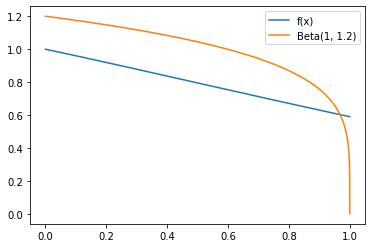
\includegraphics[scale=0.65]{beta_dist_graph.png}
\indent Apesar da queda drastica nos ultimos valores, essa distribuição mostrou otimos resultados utilizando-se de alfa = 1 e beta = 1.2
\subsubsection{Gamma}
\\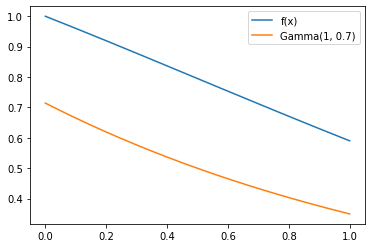
\includegraphics[scale=0.65]{gamma_dist_graph.png}
\indent O Scipy utiliza-se de outro parametro no lugar de Beta (para a distribuição Gamma), chamado Scale, onde
$scale = 1/\beta$, na legenda do grafico, esta indicado o valor de beta calculado baseado em scale, resultando em alfa = 1, beta = 0.7 e scale = 1.4
\subsubsection{Weibull}
\\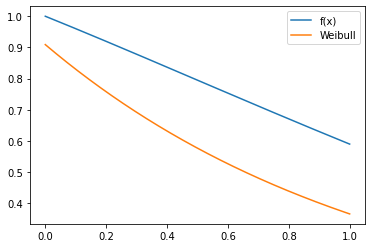
\includegraphics[scale=0.65]{weibull_dist_graph.png}
\indent Para a distribuição Weibull, utilizamos um k=1 (chamado de c, pela biblioteca que utilizei), e alteramos a escala da distribuição mexendo em seu parametro scale, atribuindo um valor de 1.1, resultando em c = k = 1 e scale = 1.1
%%%%%%%%%%%%%%%%%%%%%%
\subsection{Conclusão}
%%%%%%%%%%%%%%%%%%%%%%
Após diversos testes com os diversos métodos introduzidos por este exercicio, foi possivel obter uma comparação entre os diferentes métodos. Como todos os valores rodam pelo mesmo número de "batches" na função \textit{estimate\_error} irei apenas comparar qualitativamente os valores de N utilizados para achar erros inferiores a 0.0005 nesse exercicio. \\
\indent Em geral, os algoritmos crude e hit or miss possuem valores relativamente proximos de N (com o Crude minimamente menor)  para reduzirmos o erro, em geral por serem algoritmos que não carregam nenhuma informação do problema a priori de sua execução. \\
\indent O algoritmo de importance sampling depende muito da distribuição selecionada pelo experimentador, apesar de conseguir um otimo resultado com a distribuição Beta, não obtive resultados muito bons com as outras duas distribuições, tanto por um erro na hora de selecionar os parametros ou por sua inadequacidade ao problema referente, ainda assim, atingem o erro desejado em um N muito menor que os outros dois algoritmos. \\
\indent Por fim, o método mais eficiente (para este problema, pelo menos) foi o de Control Variates que atingiu o erro desejado em um N muito menor que todos os outros métodos, a função que desejava-se estimar possuia uma função polinomial que encaixava-se muito bem em sua distribuição, fornecendo uma informação a priori ao algoritmo que permitiu a atingir o erro desejado em poucas iterações.
\indent A baixo encontram-se os valores totais de N (multiplicando pelo numero $M$ de batches) para cada algoritmo
\begin{center}
 \begin{tabular}{||c c c c||} 
 \hline
 Algoritmo & N & M & N Total \\ [0.5ex] 
 \hline\hline
 Crude & 300000 & 100 & 30000000 \\ 
 \hline
 Hit or Miss & 400000 & 100 & 40000000 \\
 \hline
 Importance Sampling & 25000 & 100 & 2500000 \\
 \hline
 Control Variates & 1000 & 100 & 100000 \\
 \hline
\end{tabular}
\end{center}
\end{document}